\documentclass[10pt,a4paper]{article}

\usepackage[utf8x]{inputenc}
\usepackage{polski}
\usepackage{graphicx}

%\author{Mateusz Cieciura, GR 1 \\ cieciurm@ee.pw.edu.pl}
%\title{\textbf{Laboratorium Algorytmów i Struktur Danych} \\ Porównanie złożoności czasowej operacji na kopcu i liście liniowej}
\begin{document}

%\maketitle

\begin{center}
{\Large \textbf{Laboratorium Algorytmów i Struktur Danych} \\ 
Porównanie złożoności czasowej \\ operacji na kopcu i liście liniowej \\}
\vspace{20pt}
Mateusz Cieciura, GR 1 \\ cieciurm@ee.pw.edu.pl
\end{center}

\section{Wprowadzenie}

Podczas tego ćwiczenia zadaniem było zaimplementowanie kolejki priorytetowej na kopcu i posortowanej liście liniowej oraz porównanie złożoności
czasowej wstawiania elementów oraz ich usuwania.

Zgodnie z poleceniem przygotowane dane testowe to liczby naturalne od 1 do 1000, dodawane w kolejności rosnącej.

\section{Kopiec}

\subsection{Dodawanie elementów do kopca}

Na podstawie danych wyprodukowanych przez klasę testową sporządzono następujący wykres:

%\begin{figure}[hbtp]
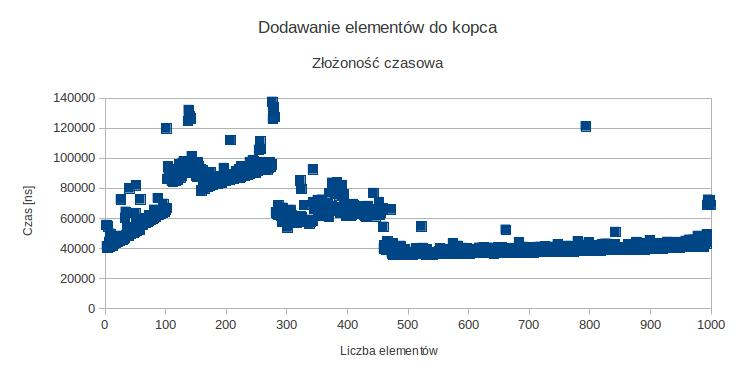
\includegraphics[scale=0.4]{heap_adding.jpg}
%\end{figure}

Można zauważyć, że na początku tj. do około 200. elementu złożoność czasowa rośnie liniowo. Następnie ma miejsce spadek
czasu i w przedziale (300;500) złożoność czasowa rośnie także liniowo. 

Dodawanie elementów od 500 do 1000 ma złożoność czasową prawie stałą, rosnącą liniowo bardzo powoli.  

\subsection{Usuwanie elementów z kopca}

%\begin{figure}[hbtp]
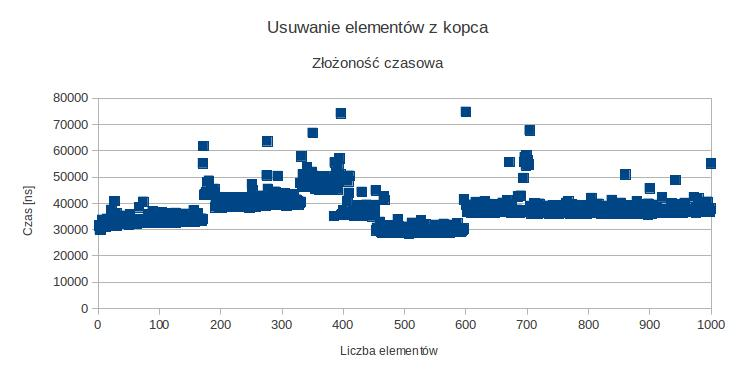
\includegraphics[scale=0.4]{heap_removing.jpg}
%\end{figure}

W przypadku usuwania elementów złożoność czasowa jest praktycznie stała, na poziomie około 40 000 nanosekund. W niektórych miejscach
przybiera kształt funkcji liniowej, ale rosnącej bardzo powoli dlatego można scharakteryzować tę funkcję jako stałą.

\section{Posortowana lista liniowa}

\subsection{Dodawanie elementów do listy}

%\begin{figure}[hbtp]
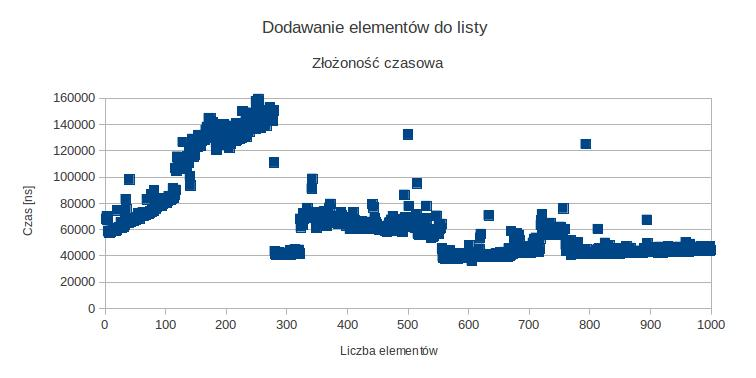
\includegraphics[scale=0.4]{list_adding.jpg}
%\end{figure}

W przypadku listy liniowej na początku złożoność czasowa jest funkcją liniową rosnącą dość szybko, dzieje się tak do mniej więcej
300. elementu. Następnie od 300 do 500 zachowuje się nieregularnie - czasami spada, ogólnie nie zmienia się gwałtowanie.

Od elementu nr 500 do ostatniego rośnie bardzo powoli, ale widać, że zachowuje się jak funkcja liniowa rosnąca.

\subsection{Usuwanie elementów z listy}

%\begin{figure}[hbtp]
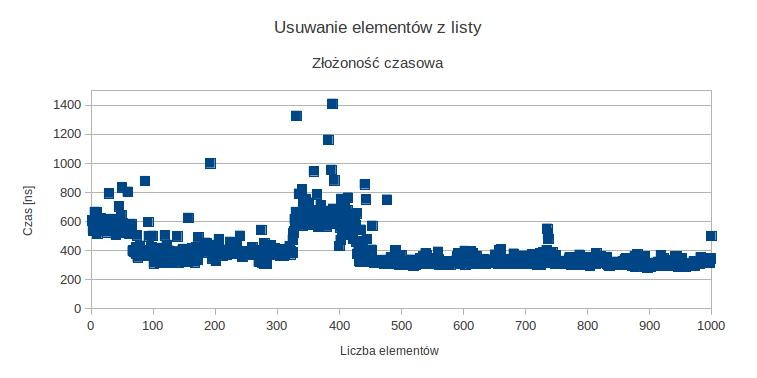
\includegraphics[scale=0.4]{list_removing.jpg}
%\end{figure}

Od samego początku widać tendencję do utrzymywania stałej wartości. Jedynie w przedziale od 300 do 400 następują gwałtowne
wzrosty i spadki. Od 400 do 1000 złożoność czasowa jest funkcją stałą. 

\section{Podsumowanie}

Na podstawie sporządzonych wykresów jest dość ciężko wyciągnąć wnioski ogólne dotyczące operacji na kopcu i posortowanej liście liniowej.
Trudno jest sformułować wnioski na temat złożoności dodawania elementów do tych struktur. Sporządzone wykresy ilustrują 
natomiast pewne charakterystyczne cechy dla usuwania z danych struktur danych oraz zależności między nimi:

\begin{itemize}
\item Złożoność usuwania elementu z posortowanej listy jest stała - dzieje się tak ponieważ największy element jest zawsze na 
początku i następuje jedynie przesunięcie wskaźnika na kolejny element. Jest to widoczne na wykresie.

\item Złożoność usuwania elementu z kopca jest także praktycznie stała - dzieje się tak ponieważ korzeniem kopca jest największy
element, więc także następuje jego natychmiastowe zwrócenie. Następnie jest konieczne uporządkowanie kopca - sprawdzenie relacji
między dziećmi i rodzicami, dlatego złożoność usuwania z kopca jest blisko 100 razy większa niż z listy.
\end{itemize} 

\end{document}